\section{Preliminaries}~\label{preliminaries}
\subsection{Symbolic State and Action Representation}~\label{preliminaries:STRIPS}
The objective of planning is to find a transition sequence that transforms the initial state into a goal state. The planning problem is defined as a tuple $\mathcal{P} = \langle \mathcal{F}, \mathcal{A}, s_0, \mathcal{G} \rangle$, where $\mathcal{F}$ is a finite set of \cp{atoms}, $\mathcal{A}$ is a set of actions, $s_0 \subseteq \mathcal{F}$ is the initial state, and $\mathcal{G} \subseteq \mathcal{F}$ is the goal condition. A state $s$ is represented as a subset of $\mathcal{F}$. Each action $a \in \mathcal{A}$ is defined as a tuple $a = \langle \mathrm{pre}(a), \mathrm{add}(a), \mathrm{del}(a) \rangle$, where $\mathrm{pre}(a), \mathrm{add}(a), \mathrm{del}(a) \subseteq \mathcal{F}$ denote the preconditions, add lists, and delete lists of the action, respectively. 
% We can say that $a$ is applicable in $s$ if and only if $\mathrm{pre}(a) \subseteq s$, denoted as $a \llbracket s \rrbracket$. 
\cp{An action $a$ is said to be applicable in state $s$ if and only if $\mathrm{pre}(a) \subseteq s$, denoted as $a \llbracket s \rrbracket$.}
The state transition is defined as $s \xrightarrow{a} s^\prime$, where $s^\prime = (s \setminus \mathrm{del}(a)) \cup \mathrm{add}(a).$

A plan is a sequence of actions $\pi = (a_1, \dots, a_T)$ such that the goal condition is satisfied after sequentially applying the actions starting from the initial state, i.e.,
\[
s_0 \xrightarrow{a_1} s_1 \xrightarrow{a_2} \cdots \xrightarrow{a_T} s_T
\quad \text{and} \quad \mathcal{G} \subseteq s_T.
\]

\subsection{POMDP}~\label{preliminaries:POMDPs}
\begin{figure}[t]
\captionsetup{skip=0pt}
    \centering
    \includegraphics[width=0.5\linewidth]
    % 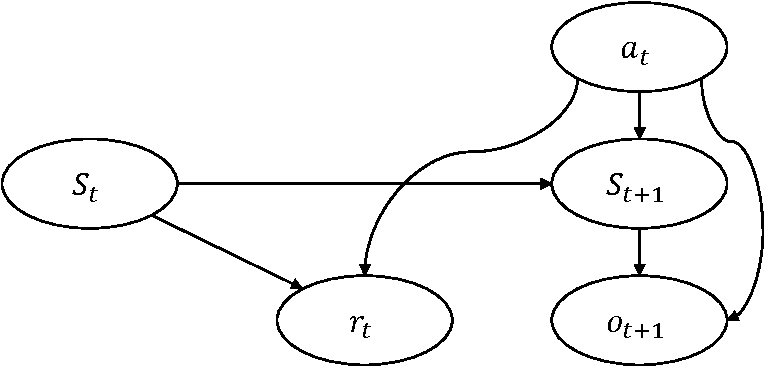
\includegraphics[width=0.85\linewidth]
    {figures/fig_pomdp_preliminaries.pdf}
    \caption{Graphical illustration of a POMDP. At each time step $t$, the agent selects an $a_t$ based on its current belief over the latent state $s_t$. The environment transitions to the next state $s_{t+1}$ and generates a reward $r_t$. Since the true state is not directly observable, the agent receives an observation $o_{t+1}$.}
    \label{fig:pomdp}
    % \vspace{-10pt}
\end{figure} 
% % In a Markov decision process (MDP), the environment is fully observable, and the agent can observe the true state at each time step. The system dynamics are defined by a transition model that specifies the probability of moving to a next state given the current state and action, along with a reward function that evaluates the outcome of actions. However, in many real-world scenarios, the true state is not directly accessible, and the agent must instead rely on partial observations.
% \cp{Markov Decision Processes (MDPs) assume full observability, but in many real-world scenarios the true state is only partially observable. In such cases, POMDPs are used to model observation uncertainty.}
% A POMDP is defined as a tuple \cp{$\mathcal{M} = \langle \mathcal{S}, \mathcal{A}, T, R, \Omega, O \rangle$}, 
% as shown in Fig.~\ref{fig:pomdp}, where $\mathcal{S}$ is the state space, $\mathcal{A}$ is the action space, and $\mathcal{O}$ is the observation space. $P(s^\prime \mid s,a)$ denotes the transition model, $O(o \mid s^\prime, a)$ the observation model, $R(s,a,s^\prime)$ the reward function, and $\gamma \in (0,1]$ the discount factor.
% Since the true state is not directly observable, the agent maintains a belief $b$, which is a probability distribution over $\mathcal{S}$ such that $b(s) = \Pr(s)$. After executing an action $a$ and receiving an observation $o$, the belief is updated according to the Bayes filter:

\cp{A POMDP is defined as a tuple $\langle \mathcal{S}, \mathcal{A}, T, R, \Omega, O, \gamma \rangle$, where $\mathcal{S}$ is the state space, $\mathcal{A}$ is the action space, and $\Omega$ is the observation space. The transition model $T(s^\prime \mid s, a)$ specifies the probability of reaching the next state $s^\prime$ after taking action $a$ in current state $s$. The observation model $O(o \mid s^\prime, a)$ defines the probability of receiving observation $o$ after arriving at state $s^\prime$ by executing action $a$. The reward function $R(s,a)$ gives a scalar value to each transition, and $\gamma \in (0,1]$ is the discount factor.

Since the true state is not directly observable, the agent maintains a belief $b$, which is a probability distribution over $\mathcal{S}$ such that $b(s) = \Pr(s)$. After executing an action $a$ and receiving an observation $o$, the belief is updated using a Bayes filter.
\begin{equation}~\label{eq:bayes_inference}
b^\prime(s^\prime) = \eta \, O(o \mid s^\prime,a) \sum_{s \in \mathcal{S}} P(s^\prime \mid s,a) \, b(s),
\end{equation}
where $\eta$ is a normalization constant.}

A policy $\pi$ maps beliefs to actions. The objective of a POMDP is to find a policy that maximizes the expected cumulative discounted reward, defined as $\mathbb{E}\left[\sum_{t=0}^{\infty} \gamma^t r_t \right]$.


\subsection{POMCP}~\label{preliminaries:POMCP}
Partially Observable Monte Carlo Planning (POMCP) performs Monte Carlo tree search over action-observation histories $h = \langle a_1 o_1 \dots a_t o_t \rangle$, where each node in the search tree corresponds to a history. Action selection follows the UCB rule:
\begin{equation}~\label{eq:ucb}
a^* = \arg\max_a \left( V(ha) + c \sqrt{\frac{\log N(h)}{N(ha)}} \right),
\end{equation}
where $V(ha)$ is the estimated value of $a$ after $h$, $N(h)$ and $N(ha)$ denote visit counts, and $c$ is an exploration constant.

Each simulation samples the next state, observation, and reward from a generative model $(s^\prime, o, r) \sim \mathcal{G}(s,a)$. The return is computed recursively as $R = r + \gamma R^\prime$, where $R^\prime$ is the return from subsequent steps. The value estimate is updated using an incremental average:
\begin{equation}~\label{eq:value_update}
V(ha) \leftarrow V(ha) + \frac{R - V(ha)}{N(ha)}.
\end{equation}

The belief associated with a history $h$ is represented implicitly as a set of particles, $B(h) = \{ s \mid s \text{ is visited at } h \}$, which approximates the posterior over states without explicit belief updates.

